\chapter{Truy vấn đoạn}

\index{truy vấn đoạn}
\index{truy vấn tổng}
\index{truy vấn min}
\index{truy vấn max}

Trong chương này, chúng ta sẽ thảo luận về các cấu trúc dữ liệu
cho phép chúng ta xử lý hiệu quả các truy vấn đoạn.
Trong một \key{truy vấn đoạn} (range query),
nhiệm vụ của chúng ta là tính toán một giá trị
dựa trên một mảng con của một mảng.
Các truy vấn đoạn điển hình là:
\begin{itemize}
\item $\texttt{sum}_q(a,b)$: tính tổng các giá trị trong đoạn $[a,b]$
\item $\texttt{min}_q(a,b)$: tìm giá trị nhỏ nhất trong đoạn $[a,b]$
\item $\texttt{max}_q(a,b)$: tìm giá trị lớn nhất trong đoạn $[a,b]$
\end{itemize}

Ví dụ, hãy xem xét đoạn $[3,6]$ trong mảng sau:
\begin{center}
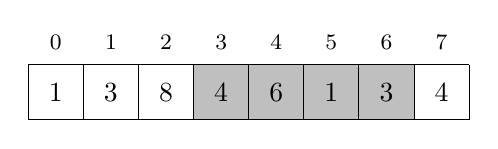
\begin{tikzpicture}[scale=0.7]
\fill[color=lightgray] (3,0) rectangle (7,1);
\draw (0,0) grid (8,1);

\node at (0.5,0.5) {$1$};
\node at (1.5,0.5) {$3$};
\node at (2.5,0.5) {$8$};
\node at (3.5,0.5) {$4$};
\node at (4.5,0.5) {$6$};
\node at (5.5,0.5) {$1$};
\node at (6.5,0.5) {$3$};
\node at (7.5,0.5) {$4$};

\footnotesize
\node at (0.5,1.4) {$0$};
\node at (1.5,1.4) {$1$};
\node at (2.5,1.4) {$2$};
\node at (3.5,1.4) {$3$};
\node at (4.5,1.4) {$4$};
\node at (5.5,1.4) {$5$};
\node at (6.5,1.4) {$6$};
\node at (7.5,1.4) {$7$};
\end{tikzpicture}
\end{center}
Trong trường hợp này, $\texttt{sum}_q(3,6)=14$,
$\texttt{min}_q(3,6)=1$ và $\texttt{max}_q(3,6)=6$.

Một cách đơn giản để xử lý các truy vấn đoạn là sử dụng
một vòng lặp duyệt qua tất cả các giá trị của mảng trong đoạn đó.
Ví dụ, hàm sau có thể được
sử dụng để xử lý các truy vấn tổng trên một mảng:

\begin{lstlisting}
int sum(int a, int b) {
    int s = 0;
    for (int i = a; i <= b; i++) {
        s += array[i];
    }
    return s;
}
\end{lstlisting}

Hàm này hoạt động trong thời gian $O(n)$,
trong đó $n$ là kích thước của mảng.
Do đó, chúng ta có thể xử lý $q$ truy vấn trong
thời gian $O(nq)$ bằng cách sử dụng hàm này.
Tuy nhiên, nếu cả $n$ và $q$ đều lớn, phương pháp này
sẽ chậm. May mắn thay, hóa ra có những
cách để xử lý các truy vấn đoạn hiệu quả hơn nhiều.

\section{Truy vấn trên mảng tĩnh}

Trước tiên, chúng ta tập trung vào một tình huống mà
mảng là \emph{tĩnh}, tức là,
các giá trị của mảng không bao giờ được cập nhật giữa các truy vấn.
Trong trường hợp này, chỉ cần xây dựng
một cấu trúc dữ liệu tĩnh cho chúng ta
câu trả lời cho bất kỳ truy vấn nào có thể có.

\subsubsection{Truy vấn tổng}

\index{mảng tổng tiền tố}

Chúng ta có thể dễ dàng xử lý
các truy vấn tổng trên một mảng tĩnh
bằng cách xây dựng một \key{mảng tổng tiền tố} (prefix sum array).
Mỗi giá trị trong mảng tổng tiền tố bằng
tổng các giá trị trong mảng ban đầu cho đến vị trí đó,
tức là, giá trị tại vị trí $k$ là $\texttt{sum}_q(0,k)$.
Mảng tổng tiền tố có thể được xây dựng trong thời gian $O(n)$.

Ví dụ, hãy xem xét mảng sau:
\begin{center}
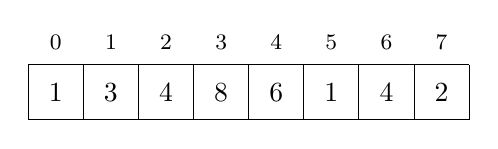
\begin{tikzpicture}[scale=0.7]
%\fill[color=lightgray] (3,0) rectangle (7,1);
\draw (0,0) grid (8,1);

\node at (0.5,0.5) {$1$};
\node at (1.5,0.5) {$3$};
\node at (2.5,0.5) {$4$};
\node at (3.5,0.5) {$8$};
\node at (4.5,0.5) {$6$};
\node at (5.5,0.5) {$1$};
\node at (6.5,0.5) {$4$};
\node at (7.5,0.5) {$2$};

\footnotesize
\node at (0.5,1.4) {$0$};
\node at (1.5,1.4) {$1$};
\node at (2.5,1.4) {$2$};
\node at (3.5,1.4) {$3$};
\node at (4.5,1.4) {$4$};
\node at (5.5,1.4) {$5$};
\node at (6.5,1.4) {$6$};
\node at (7.5,1.4) {$7$};
\end{tikzpicture}
\end{center}
Mảng tổng tiền tố tương ứng như sau:
\begin{center}
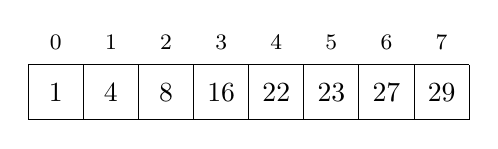
\begin{tikzpicture}[scale=0.7]
%\fill[color=lightgray] (3,0) rectangle (7,1);
\draw (0,0) grid (8,1);

\node at (0.5,0.5) {$1$};
\node at (1.5,0.5) {$4$};
\node at (2.5,0.5) {$8$};
\node at (3.5,0.5) {$16$};
\node at (4.5,0.5) {$22$};
\node at (5.5,0.5) {$23$};
\node at (6.5,0.5) {$27$};
\node at (7.5,0.5) {$29$};


\footnotesize
\node at (0.5,1.4) {$0$};
\node at (1.5,1.4) {$1$};
\node at (2.5,1.4) {$2$};
\node at (3.5,1.4) {$3$};
\node at (4.5,1.4) {$4$};
\node at (5.5,1.4) {$5$};
\node at (6.5,1.4) {$6$};
\node at (7.5,1.4) {$7$};
\end{tikzpicture}
\end{center}
Vì mảng tổng tiền tố chứa tất cả các giá trị
của $\texttt{sum}_q(0,k)$,
chúng ta có thể tính bất kỳ giá trị nào của
$\texttt{sum}_q(a,b)$ trong thời gian $O(1)$ như sau:
\[ \texttt{sum}_q(a,b) = \texttt{sum}_q(0,b) - \texttt{sum}_q(0,a-1)\]
Bằng cách định nghĩa $\texttt{sum}_q(0,-1)=0$,
công thức trên cũng đúng khi $a=0$.

Ví dụ, hãy xem xét đoạn $[3,6]$:
\begin{center}
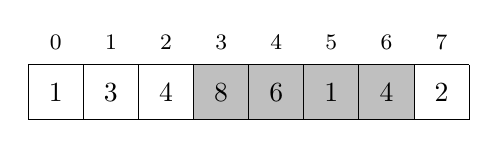
\begin{tikzpicture}[scale=0.7]
\fill[color=lightgray] (3,0) rectangle (7,1);
\draw (0,0) grid (8,1);

\node at (0.5,0.5) {$1$};
\node at (1.5,0.5) {$3$};
\node at (2.5,0.5) {$4$};
\node at (3.5,0.5) {$8$};
\node at (4.5,0.5) {$6$};
\node at (5.5,0.5) {$1$};
\node at (6.5,0.5) {$4$};
\node at (7.5,0.5) {$2$};

\footnotesize
\node at (0.5,1.4) {$0$};
\node at (1.5,1.4) {$1$};
\node at (2.5,1.4) {$2$};
\node at (3.5,1.4) {$3$};
\node at (4.5,1.4) {$4$};
\node at (5.5,1.4) {$5$};
\node at (6.5,1.4) {$6$};
\node at (7.5,1.4) {$7$};
\end{tikzpicture}
\end{center}
Trong trường hợp này $\texttt{sum}_q(3,6)=8+6+1+4=19$.
Tổng này có thể được tính từ
hai giá trị của mảng tổng tiền tố:
\begin{center}
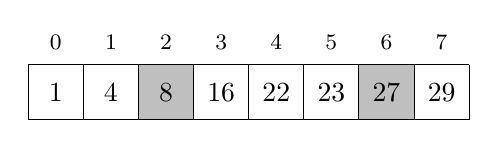
\begin{tikzpicture}[scale=0.7]
\fill[color=lightgray] (2,0) rectangle (3,1);
\fill[color=lightgray] (6,0) rectangle (7,1);
\draw (0,0) grid (8,1);

\node at (0.5,0.5) {$1$};
\node at (1.5,0.5) {$4$};
\node at (2.5,0.5) {$8$};
\node at (3.5,0.5) {$16$};
\node at (4.5,0.5) {$22$};
\node at (5.5,0.5) {$23$};
\node at (6.5,0.5) {$27$};
\node at (7.5,0.5) {$29$};

\footnotesize
\node at (0.5,1.4) {$0$};
\node at (1.5,1.4) {$1$};
\node at (2.5,1.4) {$2$};
\node at (3.5,1.4) {$3$};
\node at (4.5,1.4) {$4$};
\node at (5.5,1.4) {$5$};
\node at (6.5,1.4) {$6$};
\node at (7.5,1.4) {$7$};
\end{tikzpicture}
\end{center}
Do đó, $\texttt{sum}_q(3,6)=\texttt{sum}_q(0,6)-\texttt{sum}_q(0,2)=27-8=19$.

Cũng có thể tổng quát hóa ý tưởng này
lên các chiều cao hơn.
Ví dụ, chúng ta có thể xây dựng một
mảng tổng tiền tố hai chiều có thể được sử dụng để tính
tổng của bất kỳ mảng con hình chữ nhật nào trong thời gian $O(1)$.
Mỗi tổng trong một mảng như vậy tương ứng với
một mảng con
bắt đầu từ góc trên bên trái của mảng.

\begin{samepage}
Hình ảnh sau đây minh họa ý tưởng:
\begin{center}
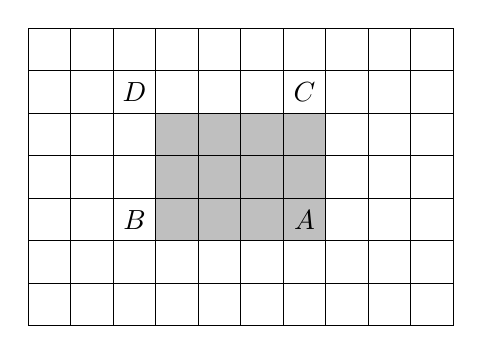
\begin{tikzpicture}[scale=0.54]
\draw[fill=lightgray] (3,2) rectangle (7,5);
\draw (0,0) grid (10,7);
\node[anchor=center] at (6.5, 2.5) {$A$};
\node[anchor=center] at (2.5, 2.5) {$B$};
\node[anchor=center] at (6.5, 5.5) {$C$};
\node[anchor=center] at (2.5, 5.5) {$D$};
\end{tikzpicture}
\end{center}
\end{samepage}

Tổng của mảng con màu xám có thể được tính
bằng công thức
\[S(A) - S(B) - S(C) + S(D),\]
trong đó $S(X)$ biểu thị tổng các giá trị
trong một mảng con hình chữ nhật
từ góc trên bên trái
đến vị trí của $X$.

\subsubsection{Truy vấn min}

\index{sparse table}

Truy vấn min khó xử lý hơn
truy vấn tổng.
Tuy nhiên, có một phương pháp tiền xử lý
khá đơn giản với thời gian $O(n \log n)$
sau đó chúng ta có thể trả lời bất kỳ truy vấn
min nào trong thời gian $O(1)$\footnote{Kỹ thuật này
được giới thiệu trong \cite{ben00} và đôi khi
được gọi là phương pháp \key{sparse table}.
Cũng có những kỹ thuật phức tạp hơn \cite{fis06} mà
thời gian tiền xử lý chỉ là $O(n)$, nhưng những thuật toán
như vậy không cần thiết trong lập trình thi đấu.}.
Lưu ý rằng vì các truy vấn min và max có thể
được xử lý tương tự nhau,
chúng ta có thể tập trung vào các truy vấn min.

Ý tưởng là tính toán trước tất cả các giá trị của
$\textrm{min}_q(a,b)$ trong đó
$b-a+1$ (độ dài của đoạn) là một lũy thừa của hai.
Ví dụ, đối với mảng

\begin{center}
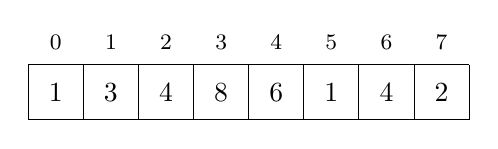
\begin{tikzpicture}[scale=0.7]
\draw (0,0) grid (8,1);

\node at (0.5,0.5) {$1$};
\node at (1.5,0.5) {$3$};
\node at (2.5,0.5) {$4$};
\node at (3.5,0.5) {$8$};
\node at (4.5,0.5) {$6$};
\node at (5.5,0.5) {$1$};
\node at (6.5,0.5) {$4$};
\node at (7.5,0.5) {$2$};

\footnotesize
\node at (0.5,1.4) {$0$};
\node at (1.5,1.4) {$1$};
\node at (2.5,1.4) {$2$};
\node at (3.5,1.4) {$3$};
\node at (4.5,1.4) {$4$};
\node at (5.5,1.4) {$5$};
\node at (6.5,1.4) {$6$};
\node at (7.5,1.4) {$7$};
\end{tikzpicture}
\end{center}
các giá trị sau được tính toán:

\begin{center}
\begin{tabular}{ccc}

\begin{tabular}{lll}
$a$ & $b$ & $\texttt{min}_q(a,b)$ \\
\hline
0 & 0 & 1 \\
1 & 1 & 3 \\
2 & 2 & 4 \\
3 & 3 & 8 \\
4 & 4 & 6 \\
5 & 5 & 1 \\
6 & 6 & 4 \\
7 & 7 & 2 \\
\end{tabular}

&

\begin{tabular}{lll}
$a$ & $b$ & $\texttt{min}_q(a,b)$ \\
\hline
0 & 1 & 1 \\
1 & 2 & 3 \\
2 & 3 & 4 \\
3 & 4 & 6 \\
4 & 5 & 1 \\
5 & 6 & 1 \\
6 & 7 & 2 \\
\\
\end{tabular}

&

\begin{tabular}{lll}
$a$ & $b$ & $\texttt{min}_q(a,b)$ \\
\hline
0 & 3 & 1 \\
1 & 4 & 3 \\
2 & 5 & 1 \\
3 & 6 & 1 \\
4 & 7 & 1 \\
0 & 7 & 1 \\
\\
\\
\end{tabular}

\end{tabular}
\end{center}

Số lượng các giá trị được tính toán trước là $O(n \log n)$,
bởi vì có $O(\log n)$ độ dài đoạn
là lũy thừa của hai.
Các giá trị có thể được tính toán hiệu quả
bằng công thức đệ quy
\[\texttt{min}_q(a,b) = \min(\texttt{min}_q(a,a+w-1),\texttt{min}_q(a+w,b)),\]
trong đó $b-a+1$ là một lũy thừa của hai và $w=(b-a+1)/2$.
Tính toán tất cả các giá trị đó mất thời gian $O(n \log n)$.

Sau đó, bất kỳ giá trị nào của $\texttt{min}_q(a,b)$ có thể được tính
trong thời gian $O(1)$ như là giá trị nhỏ nhất của hai giá trị đã được tính toán trước.
Gọi $k$ là lũy thừa lớn nhất của hai không vượt quá $b-a+1$.
Chúng ta có thể tính giá trị của $\texttt{min}_q(a,b)$ bằng công thức
\[\texttt{min}_q(a,b) = \min(\texttt{min}_q(a,a+k-1),\texttt{min}_q(b-k+1,b)).\]
Trong công thức trên, đoạn $[a,b]$ được biểu diễn
như là hợp của các đoạn $[a,a+k-1]$ và $[b-k+1,b]$, cả hai đều có độ dài $k$.

Ví dụ, hãy xem xét đoạn $[1,6]$:
\begin{center}
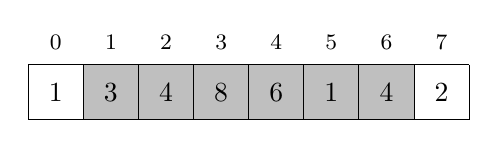
\begin{tikzpicture}[scale=0.7]
\fill[color=lightgray] (1,0) rectangle (7,1);
\draw (0,0) grid (8,1);

\node at (0.5,0.5) {$1$};
\node at (1.5,0.5) {$3$};
\node at (2.5,0.5) {$4$};
\node at (3.5,0.5) {$8$};
\node at (4.5,0.5) {$6$};
\node at (5.5,0.5) {$1$};
\node at (6.5,0.5) {$4$};
\node at (7.5,0.5) {$2$};

\footnotesize
\node at (0.5,1.4) {$0$};
\node at (1.5,1.4) {$1$};
\node at (2.5,1.4) {$2$};
\node at (3.5,1.4) {$3$};
\node at (4.5,1.4) {$4$};
\node at (5.5,1.4) {$5$};
\node at (6.5,1.4) {$6$};
\node at (7.5,1.4) {$7$};
\end{tikzpicture}
\end{center}
Độ dài của đoạn là 6,
và lũy thừa lớn nhất của hai không
vượt quá 6 là 4.
Do đó, đoạn $[1,6]$ là
hợp của các đoạn $[1,4]$ và $[3,6]$:
\begin{center}
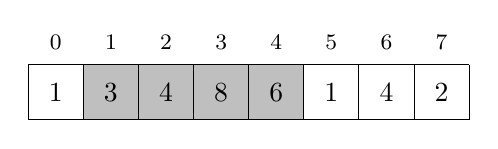
\begin{tikzpicture}[scale=0.7]
\fill[color=lightgray] (1,0) rectangle (5,1);
\draw (0,0) grid (8,1);

\node at (0.5,0.5) {$1$};
\node at (1.5,0.5) {$3$};
\node at (2.5,0.5) {$4$};
\node at (3.5,0.5) {$8$};
\node at (4.5,0.5) {$6$};
\node at (5.5,0.5) {$1$};
\node at (6.5,0.5) {$4$};
\node at (7.5,0.5) {$2$};

\footnotesize
\node at (0.5,1.4) {$0$};
\node at (1.5,1.4) {$1$};
\node at (2.5,1.4) {$2$};
\node at (3.5,1.4) {$3$};
\node at (4.5,1.4) {$4$};
\node at (5.5,1.4) {$5$};
\node at (6.5,1.4) {$6$};
\node at (7.5,1.4) {$7$};
\end{tikzpicture}
\end{center}
\begin{center}
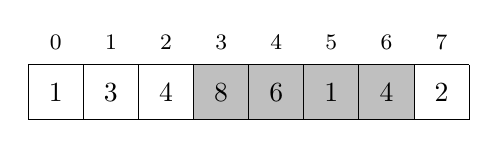
\begin{tikzpicture}[scale=0.7]
\fill[color=lightgray] (3,0) rectangle (7,1);
\draw (0,0) grid (8,1);

\node at (0.5,0.5) {$1$};
\node at (1.5,0.5) {$3$};
\node at (2.5,0.5) {$4$};
\node at (3.5,0.5) {$8$};
\node at (4.5,0.5) {$6$};
\node at (5.5,0.5) {$1$};
\node at (6.5,0.5) {$4$};
\node at (7.5,0.5) {$2$};


\footnotesize
\node at (0.5,1.4) {$0$};
\node at (1.5,1.4) {$1$};
\node at (2.5,1.4) {$2$};
\node at (3.5,1.4) {$3$};
\node at (4.5,1.4) {$4$};
\node at (5.5,1.4) {$5$};
\node at (6.5,1.4) {$6$};
\node at (7.5,1.4) {$7$};
\end{tikzpicture}
\end{center}
Vì $\texttt{min}_q(1,4)=3$ và $\texttt{min}_q(3,6)=1$,
chúng ta kết luận rằng $\texttt{min}_q(1,6)=1$.

\section{Cây chỉ số nhị phân (Binary indexed tree)}

\index{cây chỉ số nhị phân}
\index{cây Fenwick}

Một \key{cây chỉ số nhị phân} (binary indexed tree) hay một \key{cây Fenwick}\footnote{Cấu trúc
cây chỉ số nhị phân được trình bày bởi P. M. Fenwick vào năm 1994 \cite{fen94}.}
có thể được xem như một biến thể động của mảng tổng tiền tố.
Nó hỗ trợ hai thao tác thời gian $O(\log n)$ trên một mảng:
xử lý một truy vấn tổng đoạn và cập nhật một giá trị.

Ưu điểm của một cây chỉ số nhị phân là
nó cho phép chúng ta cập nhật hiệu quả
các giá trị của mảng giữa các truy vấn tổng.
Điều này sẽ không thể thực hiện được bằng cách sử dụng một mảng tổng tiền tố,
bởi vì sau mỗi lần cập nhật, sẽ cần phải xây dựng lại
toàn bộ mảng tổng tiền tố trong thời gian $O(n)$.

\subsubsection{Cấu trúc}

Mặc dù tên của cấu trúc là một \emph{cây} chỉ số nhị phân,
nó thường được biểu diễn dưới dạng một mảng.
Trong phần này, chúng ta giả định rằng tất cả các mảng đều được đánh chỉ số từ một,
bởi vì nó làm cho việc cài đặt dễ dàng hơn.

Gọi $p(k)$ là lũy thừa lớn nhất của hai mà
chia hết cho $k$.
Chúng ta lưu trữ một cây chỉ số nhị phân dưới dạng một mảng \texttt{tree}
sao cho
\[ \texttt{tree}[k] = \texttt{sum}_q(k-p(k)+1,k),\]
tức là, mỗi vị trí $k$ chứa tổng các giá trị
trong một đoạn của mảng ban đầu có độ dài là $p(k)$
và kết thúc tại vị trí $k$.
Ví dụ, vì $p(6)=2$, $\texttt{tree}[6]$
chứa giá trị của $\texttt{sum}_q(5,6)$.

Ví dụ, hãy xem xét mảng sau:
\begin{center}
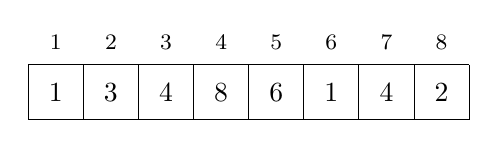
\begin{tikzpicture}[scale=0.7]
\draw (0,0) grid (8,1);

\node at (0.5,0.5) {$1$};
\node at (1.5,0.5) {$3$};
\node at (2.5,0.5) {$4$};
\node at (3.5,0.5) {$8$};
\node at (4.5,0.5) {$6$};
\node at (5.5,0.5) {$1$};
\node at (6.5,0.5) {$4$};
\node at (7.5,0.5) {$2$};

\footnotesize
\node at (0.5,1.4) {$1$};
\node at (1.5,1.4) {$2$};
\node at (2.5,1.4) {$3$};
\node at (3.5,1.4) {$4$};
\node at (4.5,1.4) {$5$};
\node at (5.5,1.4) {$6$};
\node at (6.5,1.4) {$7$};
\node at (7.5,1.4) {$8$};
\end{tikzpicture}
\end{center}

Cây chỉ số nhị phân tương ứng như sau:
\begin{center}
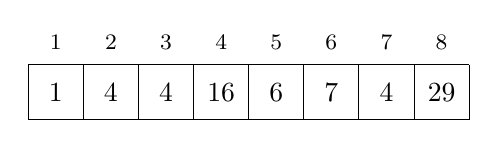
\begin{tikzpicture}[scale=0.7]
\draw (0,0) grid (8,1);

\node at (0.5,0.5) {$1$};
\node at (1.5,0.5) {$4$};
\node at (2.5,0.5) {$4$};
\node at (3.5,0.5) {$16$};
\node at (4.5,0.5) {$6$};
\node at (5.5,0.5) {$7$};
\node at (6.5,0.5) {$4$};
\node at (7.5,0.5) {$29$};

\footnotesize
\node at (0.5,1.4) {$1$};
\node at (1.5,1.4) {$2$};
\node at (2.5,1.4) {$3$};
\node at (3.5,1.4) {$4$};
\node at (4.5,1.4) {$5$};
\node at (5.5,1.4) {$6$};
\node at (6.5,1.4) {$7$};
\node at (7.5,1.4) {$8$};
\end{tikzpicture}
\end{center}

Hình ảnh sau đây cho thấy rõ hơn
cách mỗi giá trị trong cây chỉ số nhị phân
tương ứng với một đoạn trong mảng ban đầu:

\begin{center}
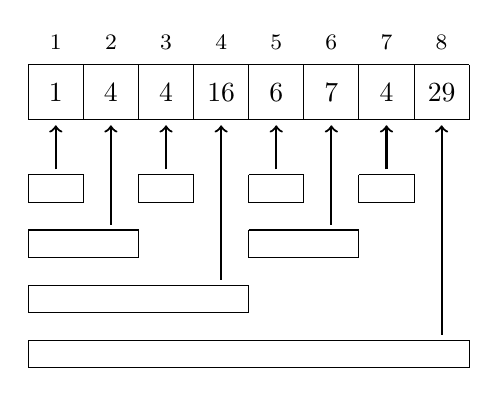
\begin{tikzpicture}[scale=0.7]
\draw (0,0) grid (8,1);

\node at (0.5,0.5) {$1$};
\node at (1.5,0.5) {$4$};
\node at (2.5,0.5) {$4$};
\node at (3.5,0.5) {$16$};
\node at (4.5,0.5) {$6$};
\node at (5.5,0.5) {$7$};
\node at (6.5,0.5) {$4$};
\node at (7.5,0.5) {$29$};

\footnotesize
\node at (0.5,1.4) {$1$};
\node at (1.5,1.4) {$2$};
\node at (2.5,1.4) {$3$};
\node at (3.5,1.4) {$4$};
\node at (4.5,1.4) {$5$};
\node at (5.5,1.4) {$6$};
\node at (6.5,1.4) {$7$};
\node at (7.5,1.4) {$8$};

\draw[->,thick] (0.5,-0.9) -- (0.5,-0.1);
\draw[->,thick] (2.5,-0.9) -- (2.5,-0.1);
\draw[->,thick] (4.5,-0.9) -- (4.5,-0.1);
\draw[->,thick] (6.5,-0.9) -- (6.5,-0.1);
\draw[->,thick] (1.5,-1.9) -- (1.5,-0.1);
\draw[->,thick] (5.5,-1.9) -- (5.5,-0.1);
\draw[->,thick] (3.5,-2.9) -- (3.5,-0.1);
\draw[->,thick] (7.5,-3.9) -- (7.5,-0.1);

\draw (0,-1) -- (1,-1) -- (1,-1.5) -- (0,-1.5) -- (0,-1);
\draw (2,-1) -- (3,-1) -- (3,-1.5) -- (2,-1.5) -- (2,-1);
\draw (4,-1) -- (5,-1) -- (5,-1.5) -- (4,-1.5) -- (4,-1);
\draw (6,-1) -- (7,-1) -- (7,-1.5) -- (6,-1.5) -- (6,-1);
\draw (0,-2) -- (2,-2) -- (2,-2.5) -- (0,-2.5) -- (0,-2);
\draw (4,-2) -- (6,-2) -- (6,-2.5) -- (4,-2.5) -- (4,-2);
\draw (0,-3) -- (4,-3) -- (4,-3.5) -- (0,-3.5) -- (0,-3);
\draw (0,-4) -- (8,-4) -- (8,-4.5) -- (0,-4.5) -- (0,-4);
\end{tikzpicture}
\end{center}

Sử dụng một cây chỉ số nhị phân,
bất kỳ giá trị nào của $\texttt{sum}_q(1,k)$
đều có thể được tính trong thời gian $O(\log n)$,
bởi vì một đoạn $[1,k]$ luôn có thể được chia thành
$O(\log n)$ đoạn mà tổng của chúng được lưu trữ trong cây.

Ví dụ, đoạn $[1,7]$ bao gồm
các đoạn sau:
\begin{center}
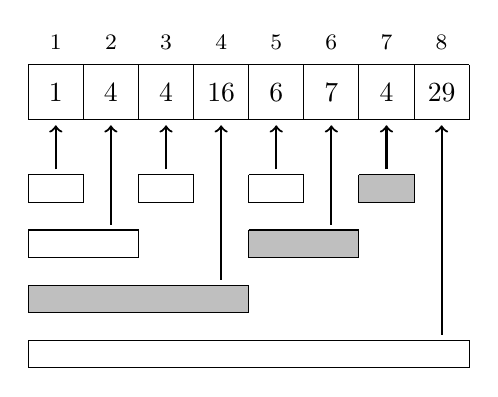
\begin{tikzpicture}[scale=0.7]
\draw (0,0) grid (8,1);

\node at (0.5,0.5) {$1$};
\node at (1.5,0.5) {$4$};
\node at (2.5,0.5) {$4$};
\node at (3.5,0.5) {$16$};
\node at (4.5,0.5) {$6$};
\node at (5.5,0.5) {$7$};
\node at (6.5,0.5) {$4$};
\node at (7.5,0.5) {$29$};

\footnotesize
\node at (0.5,1.4) {$1$};
\node at (1.5,1.4) {$2$};
\node at (2.5,1.4) {$3$};
\node at (3.5,1.4) {$4$};
\node at (4.5,1.4) {$5$};
\node at (5.5,1.4) {$6$};
\node at (6.5,1.4) {$7$};
\node at (7.5,1.4) {$8$};

\draw[->,thick] (0.5,-0.9) -- (0.5,-0.1);
\draw[->,thick] (2.5,-0.9) -- (2.5,-0.1);
\draw[->,thick] (4.5,-0.9) -- (4.5,-0.1);
\draw[->,thick] (6.5,-0.9) -- (6.5,-0.1);
\draw[->,thick] (1.5,-1.9) -- (1.5,-0.1);
\draw[->,thick] (5.5,-1.9) -- (5.5,-0.1);
\draw[->,thick] (3.5,-2.9) -- (3.5,-0.1);
\draw[->,thick] (7.5,-3.9) -- (7.5,-0.1);

\draw (0,-1) -- (1,-1) -- (1,-1.5) -- (0,-1.5) -- (0,-1);
\draw (2,-1) -- (3,-1) -- (3,-1.5) -- (2,-1.5) -- (2,-1);
\draw (4,-1) -- (5,-1) -- (5,-1.5) -- (4,-1.5) -- (4,-1);
\draw[fill=lightgray] (6,-1) -- (7,-1) -- (7,-1.5) -- (6,-1.5) -- (6,-1);
\draw (0,-2) -- (2,-2) -- (2,-2.5) -- (0,-2.5) -- (0,-2);
\draw[fill=lightgray] (4,-2) -- (6,-2) -- (6,-2.5) -- (4,-2.5) -- (4,-2);
\draw[fill=lightgray] (0,-3) -- (4,-3) -- (4,-3.5) -- (0,-3.5) -- (0,-3);
\draw (0,-4) -- (8,-4) -- (8,-4.5) -- (0,-4.5) -- (0,-4);
\end{tikzpicture}
\end{center}
Do đó, chúng ta có thể tính tổng tương ứng như sau:
\[\texttt{sum}_q(1,7)=\texttt{sum}_q(1,4)+\texttt{sum}_q(5,6)+\texttt{sum}_q(7,7)=16+7+4=27\]

Để tính giá trị của $\texttt{sum}_q(a,b)$ trong đó $a>1$,
chúng ta có thể sử dụng mẹo tương tự mà chúng ta đã sử dụng với mảng tổng tiền tố:
\[ \texttt{sum}_q(a,b) = \texttt{sum}_q(1,b) - \texttt{sum}_q(1,a-1).\]
Vì chúng ta có thể tính cả $\texttt{sum}_q(1,b)$
và $\texttt{sum}_q(1,a-1)$ trong thời gian $O(\log n)$,
tổng độ phức tạp thời gian là $O(\log n)$.

Sau đó, sau khi cập nhật một giá trị trong mảng ban đầu,
một vài giá trị trong cây chỉ số nhị phân
cần được cập nhật.
Ví dụ, nếu giá trị tại vị trí 3 thay đổi,
tổng của các đoạn sau sẽ thay đổi:
\begin{center}
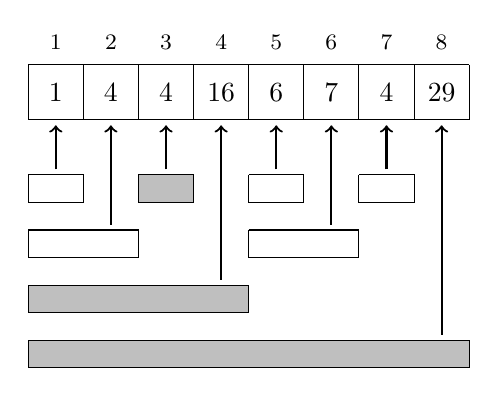
\begin{tikzpicture}[scale=0.7]
\draw (0,0) grid (8,1);

\node at (0.5,0.5) {$1$};
\node at (1.5,0.5) {$4$};
\node at (2.5,0.5) {$4$};
\node at (3.5,0.5) {$16$};
\node at (4.5,0.5) {$6$};
\node at (5.5,0.5) {$7$};
\node at (6.5,0.5) {$4$};
\node at (7.5,0.5) {$29$};

\footnotesize
\node at (0.5,1.4) {$1$};
\node at (1.5,1.4) {$2$};
\node at (2.5,1.4) {$3$};
\node at (3.5,1.4) {$4$};
\node at (4.5,1.4) {$5$};
\node at (5.5,1.4) {$6$};
\node at (6.5,1.4) {$7$};
\node at (7.5,1.4) {$8$};

\draw[->,thick] (0.5,-0.9) -- (0.5,-0.1);
\draw[->,thick] (2.5,-0.9) -- (2.5,-0.1);
\draw[->,thick] (4.5,-0.9) -- (4.5,-0.1);
\draw[->,thick] (6.5,-0.9) -- (6.5,-0.1);
\draw[->,thick] (1.5,-1.9) -- (1.5,-0.1);
\draw[->,thick] (5.5,-1.9) -- (5.5,-0.1);
\draw[->,thick] (3.5,-2.9) -- (3.5,-0.1);
\draw[->,thick] (7.5,-3.9) -- (7.5,-0.1);

\draw (0,-1) -- (1,-1) -- (1,-1.5) -- (0,-1.5) -- (0,-1);
\draw[fill=lightgray] (2,-1) -- (3,-1) -- (3,-1.5) -- (2,-1.5) -- (2,-1);
\draw (4,-1) -- (5,-1) -- (5,-1.5) -- (4,-1.5) -- (4,-1);
\draw (6,-1) -- (7,-1) -- (7,-1.5) -- (6,-1.5) -- (6,-1);
\draw (0,-2) -- (2,-2) -- (2,-2.5) -- (0,-2.5) -- (0,-2);
\draw (4,-2) -- (6,-2) -- (6,-2.5) -- (4,-2.5) -- (4,-2);
\draw[fill=lightgray] (0,-3) -- (4,-3) -- (4,-3.5) -- (0,-3.5) -- (0,-3);
\draw[fill=lightgray] (0,-4) -- (8,-4) -- (8,-4.5) -- (0,-4.5) -- (0,-4);
\end{tikzpicture}
\end{center}

Vì mỗi phần tử của mảng thuộc về $O(\log n)$
đoạn trong cây chỉ số nhị phân,
chỉ cần cập nhật $O(\log n)$ giá trị trong cây.

\subsubsection{Cài đặt}

Các thao tác của một cây chỉ số nhị phân có thể được
cài đặt hiệu quả bằng cách sử dụng các phép toán bit.
Sự thật quan trọng cần thiết là chúng ta có thể
tính bất kỳ giá trị nào của $p(k)$ bằng công thức
\[p(k) = k \& -k.\]

Hàm sau tính giá trị của $\texttt{sum}_q(1,k)$:
\begin{lstlisting}
int sum(int k) {
    int s = 0;
    while (k >= 1) {
        s += tree[k];
        k -= k&-k;
    }
    return s;
}
\end{lstlisting}

Hàm sau tăng giá trị
của mảng tại vị trí $k$ lên $x$
($x$ có thể là dương hoặc âm):
\begin{lstlisting}
void add(int k, int x) {
    while (k <= n) {
        tree[k] += x;
        k += k&-k;
    }
}
\end{lstlisting}

Độ phức tạp thời gian của cả hai hàm là
$O(\log n)$, bởi vì các hàm truy cập $O(\log n)$
giá trị trong cây chỉ số nhị phân, và mỗi lần di chuyển
đến vị trí tiếp theo mất thời gian $O(1)$.

\section{Cây đoạn (Segment tree)}

\index{cây đoạn}

Một \key{cây đoạn} (segment tree)\footnote{Việc cài đặt từ dưới lên trong chương này tương ứng với
cách trong \cite{sta06}. Các cấu trúc tương tự đã được sử dụng
vào cuối những năm 1970 để giải quyết các bài toán hình học \cite{ben80}.} là một cấu trúc dữ liệu
hỗ trợ hai thao tác:
xử lý một truy vấn đoạn và
cập nhật một giá trị của mảng.
Cây đoạn có thể hỗ trợ
các truy vấn tổng, truy vấn min và max và nhiều
truy vấn khác sao cho cả hai thao tác đều hoạt động trong thời gian $O(\log n)$.

So với một cây chỉ số nhị phân,
ưu điểm của cây đoạn là nó là
một cấu trúc dữ liệu tổng quát hơn.
Trong khi cây chỉ số nhị phân chỉ hỗ trợ
các truy vấn tổng\footnote{Thực tế, bằng cách sử dụng \emph{hai} cây
chỉ số nhị phân, có thể hỗ trợ các truy vấn min \cite{dim15},
nhưng điều này phức tạp hơn so với việc sử dụng một cây đoạn.},
cây đoạn cũng hỗ trợ các truy vấn khác.
Mặt khác, một cây đoạn yêu cầu nhiều
bộ nhớ hơn và khó cài đặt hơn một chút.

\subsubsection{Cấu trúc}

Một cây đoạn là một cây nhị phân
sao cho các nút ở tầng dưới cùng của cây
tương ứng với các phần tử của mảng,
và các nút khác
chứa thông tin cần thiết để xử lý các truy vấn đoạn.

Trong phần này, chúng ta giả định rằng kích thước
của mảng là một lũy thừa của hai và sử dụng
chỉ số dựa trên không, bởi vì việc xây dựng
một cây đoạn cho một mảng như vậy rất thuận tiện.
Nếu kích thước của mảng không phải là một lũy thừa của hai,
chúng ta luôn có thể thêm các phần tử phụ vào nó.

Đầu tiên chúng ta sẽ thảo luận về cây đoạn hỗ trợ các truy vấn tổng.
Ví dụ, hãy xem xét mảng sau:
\begin{center}
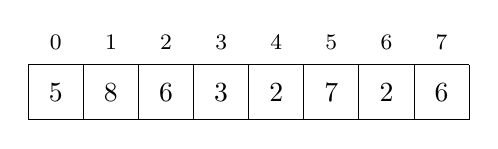
\begin{tikzpicture}[scale=0.7]
\draw (0,0) grid (8,1);

\node at (0.5,0.5) {$5$};
\node at (1.5,0.5) {$8$};
\node at (2.5,0.5) {$6$};
\node at (3.5,0.5) {$3$};
\node at (4.5,0.5) {$2$};
\node at (5.5,0.5) {$7$};
\node at (6.5,0.5) {$2$};
\node at (7.5,0.5) {$6$};

\footnotesize
\node at (0.5,1.4) {$0$};
\node at (1.5,1.4) {$1$};
\node at (2.5,1.4) {$2$};
\node at (3.5,1.4) {$3$};
\node at (4.5,1.4) {$4$};
\node at (5.5,1.4) {$5$};
\node at (6.5,1.4) {$6$};
\node at (7.5,1.4) {$7$};
\end{tikzpicture}
\end{center}
Cây đoạn tương ứng như sau:
\begin{center}
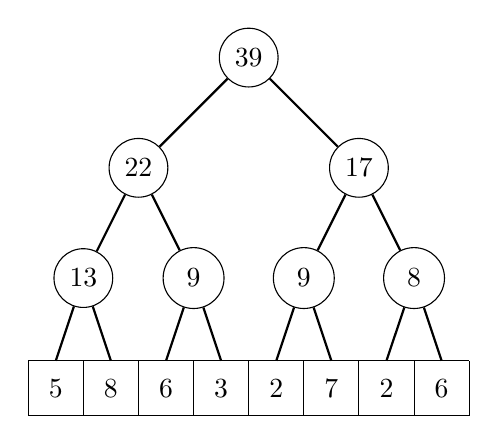
\begin{tikzpicture}[scale=0.7]
\draw (0,0) grid (8,1);

\node[anchor=center] at (0.5, 0.5) {5};
\node[anchor=center] at (1.5, 0.5) {8};
\node[anchor=center] at (2.5, 0.5) {6};
\node[anchor=center] at (3.5, 0.5) {3};
\node[anchor=center] at (4.5, 0.5) {2};
\node[anchor=center] at (5.5, 0.5) {7};
\node[anchor=center] at (6.5, 0.5) {2};
\node[anchor=center] at (7.5, 0.5) {6};

\node[draw, circle] (a) at (1,2.5) {13};
\path[draw,thick,-] (a) -- (0.5,1);
\path[draw,thick,-] (a) -- (1.5,1);
\node[draw, circle,minimum size=22pt] (b) at (3,2.5) {9};
\path[draw,thick,-] (b) -- (2.5,1);
\path[draw,thick,-] (b) -- (3.5,1);
\node[draw, circle,minimum size=22pt] (c) at (5,2.5) {9};
\path[draw,thick,-] (c) -- (4.5,1);
\path[draw,thick,-] (c) -- (5.5,1);
\node[draw, circle,minimum size=22pt] (d) at (7,2.5) {8};
\path[draw,thick,-] (d) -- (6.5,1);
\path[draw,thick,-] (d) -- (7.5,1);

\node[draw, circle] (i) at (2,4.5) {22};
\path[draw,thick,-] (i) -- (a);
\path[draw,thick,-] (i) -- (b);
\node[draw, circle] (j) at (6,4.5) {17};
\path[draw,thick,-] (j) -- (c);
\path[draw,thick,-] (j) -- (d);

\node[draw, circle] (m) at (4,6.5) {39};
\path[draw,thick,-] (m) -- (i);
\path[draw,thick,-] (m) -- (j);
\end{tikzpicture}
\end{center}

Mỗi nút trong cây
tương ứng với một đoạn của mảng
có kích thước là một lũy thừa của hai.
Trong cây trên, giá trị của mỗi nút trong
là tổng của các giá trị mảng tương ứng,
và nó có thể được tính bằng tổng của
giá trị của nút con trái và phải của nó.

Hóa ra bất kỳ đoạn nào $[a,b]$
cũng có thể được chia thành $O(\log n)$ đoạn
mà giá trị của chúng được lưu trữ trong các nút của cây.
Ví dụ, hãy xem xét đoạn [2,7]:
\begin{center}
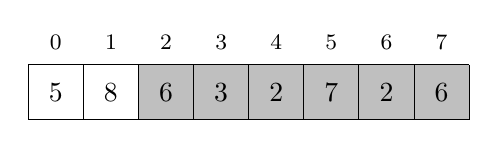
\begin{tikzpicture}[scale=0.7]
\fill[color=gray!50] (2,0) rectangle (8,1);
\draw (0,0) grid (8,1);

\node[anchor=center] at (0.5, 0.5) {5};
\node[anchor=center] at (1.5, 0.5) {8};
\node[anchor=center] at (2.5, 0.5) {6};
\node[anchor=center] at (3.5, 0.5) {3};
\node[anchor=center] at (4.5, 0.5) {2};
\node[anchor=center] at (5.5, 0.5) {7};
\node[anchor=center] at (6.5, 0.5) {2};
\node[anchor=center] at (7.5, 0.5) {6};

\footnotesize
\node at (0.5,1.4) {$0$};
\node at (1.5,1.4) {$1$};
\node at (2.5,1.4) {$2$};
\node at (3.5,1.4) {$3$};
\node at (4.5,1.4) {$4$};
\node at (5.5,1.4) {$5$};
\node at (6.5,1.4) {$6$};
\node at (7.5,1.4) {$7$};
\end{tikzpicture}
\end{center}
Ở đây $\texttt{sum}_q(2,7)=6+3+2+7+2+6=26$.
Trong trường hợp này, hai nút cây sau đây
tương ứng với đoạn đó:
\begin{center}
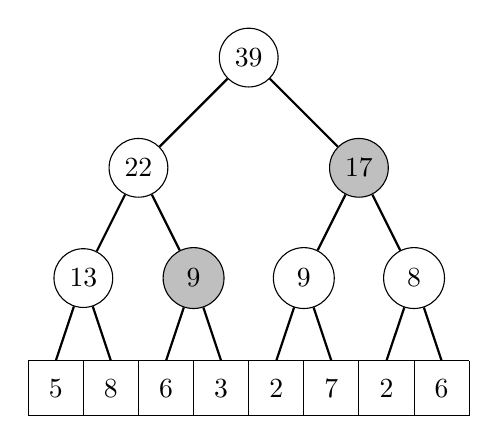
\begin{tikzpicture}[scale=0.7]
\draw (0,0) grid (8,1);

\node[anchor=center] at (0.5, 0.5) {5};
\node[anchor=center] at (1.5, 0.5) {8};
\node[anchor=center] at (2.5, 0.5) {6};
\node[anchor=center] at (3.5, 0.5) {3};
\node[anchor=center] at (4.5, 0.5) {2};
\node[anchor=center] at (5.5, 0.5) {7};
\node[anchor=center] at (6.5, 0.5) {2};
\node[anchor=center] at (7.5, 0.5) {6};

\node[draw, circle] (a) at (1,2.5) {13};
\path[draw,thick,-] (a) -- (0.5,1);
\path[draw,thick,-] (a) -- (1.5,1);
\node[draw, circle,fill=gray!50,minimum size=22pt] (b) at (3,2.5) {9};
\path[draw,thick,-] (b) -- (2.5,1);
\path[draw,thick,-] (b) -- (3.5,1);
\node[draw, circle,minimum size=22pt] (c) at (5,2.5) {9};
\path[draw,thick,-] (c) -- (4.5,1);
\path[draw,thick,-] (c) -- (5.5,1);
\node[draw, circle,minimum size=22pt] (d) at (7,2.5) {8};
\path[draw,thick,-] (d) -- (6.5,1);
\path[draw,thick,-] (d) -- (7.5,1);

\node[draw, circle] (i) at (2,4.5) {22};
\path[draw,thick,-] (i) -- (a);
\path[draw,thick,-] (i) -- (b);
\node[draw, circle,fill=gray!50] (j) at (6,4.5) {17};
\path[draw,thick,-] (j) -- (c);
\path[draw,thick,-] (j) -- (d);

\node[draw, circle] (m) at (4,6.5) {39};
\path[draw,thick,-] (m) -- (i);
\path[draw,thick,-] (m) -- (j);
\end{tikzpicture}
\end{center}
Do đó, một cách khác để tính tổng là $9+17=26$.

Khi tổng được tính bằng cách sử dụng các nút
nằm càng cao càng tốt trong cây,
cần nhiều nhất hai nút ở mỗi tầng
của cây.
Do đó, tổng số nút
là $O(\log n)$.

Sau khi cập nhật mảng,
chúng ta nên cập nhật tất cả các nút
mà giá trị của chúng phụ thuộc vào giá trị được cập nhật.
Điều này có thể được thực hiện bằng cách đi theo đường
từ phần tử mảng được cập nhật đến nút gốc
và cập nhật các nút dọc theo đường đi.

Hình ảnh sau đây cho thấy những nút cây nào
thay đổi nếu giá trị 7 của mảng thay đổi:

\begin{center}
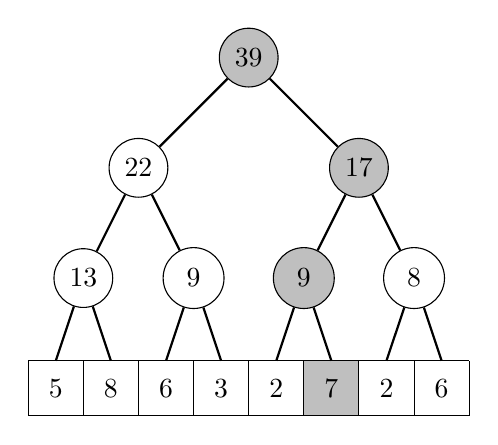
\begin{tikzpicture}[scale=0.7]
\fill[color=gray!50] (5,0) rectangle (6,1);
\draw (0,0) grid (8,1);

\node[anchor=center] at (0.5, 0.5) {5};
\node[anchor=center] at (1.5, 0.5) {8};
\node[anchor=center] at (2.5, 0.5) {6};
\node[anchor=center] at (3.5, 0.5) {3};
\node[anchor=center] at (4.5, 0.5) {2};
\node[anchor=center] at (5.5, 0.5) {7};
\node[anchor=center] at (6.5, 0.5) {2};
\node[anchor=center] at (7.5, 0.5) {6};

\node[draw, circle] (a) at (1,2.5) {13};
\path[draw,thick,-] (a) -- (0.5,1);
\path[draw,thick,-] (a) -- (1.5,1);
\node[draw, circle,minimum size=22pt] (b) at (3,2.5) {9};
\path[draw,thick,-] (b) -- (2.5,1);
\path[draw,thick,-] (b) -- (3.5,1);
\node[draw, circle,minimum size=22pt,fill=gray!50] (c) at (5,2.5) {9};
\path[draw,thick,-] (c) -- (4.5,1);
\path[draw,thick,-] (c) -- (5.5,1);
\node[draw, circle,minimum size=22pt] (d) at (7,2.5) {8};
\path[draw,thick,-] (d) -- (6.5,1);
\path[draw,thick,-] (d) -- (7.5,1);

\node[draw, circle] (i) at (2,4.5) {22};
\path[draw,thick,-] (i) -- (a);
\path[draw,thick,-] (i) -- (b);
\node[draw, circle,fill=gray!50] (j) at (6,4.5) {17};
\path[draw,thick,-] (j) -- (c);
\path[draw,thick,-] (j) -- (d);

\node[draw, circle,fill=gray!50] (m) at (4,6.5) {39};
\path[draw,thick,-] (m) -- (i);
\path[draw,thick,-] (m) -- (j);
\end{tikzpicture}
\end{center}

Đường đi từ dưới lên trên
luôn bao gồm $O(\log n)$ nút,
vì vậy mỗi lần cập nhật thay đổi $O(\log n)$ nút trong cây.

\subsubsection{Cài đặt}

Chúng ta lưu trữ một cây đoạn dưới dạng một mảng
gồm $2n$ phần tử, trong đó $n$ là kích thước của
mảng ban đầu và là một lũy thừa của hai.
Các nút của cây được lưu trữ từ trên xuống dưới:
$\texttt{tree}[1]$ là nút gốc,
$\texttt{tree}[2]$ và $\texttt{tree}[3]$
là các con của nó, và cứ thế.
Cuối cùng, các giá trị từ $\texttt{tree}[n]$
đến $\texttt{tree}[2n-1]$ tương ứng với
các giá trị của mảng ban đầu
ở tầng dưới cùng của cây.

Ví dụ, cây đoạn
\begin{center}
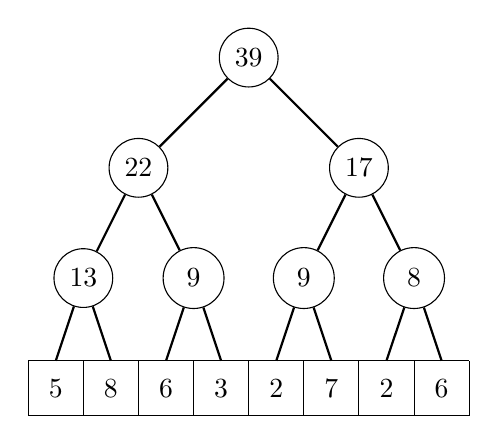
\begin{tikzpicture}[scale=0.7]
\draw (0,0) grid (8,1);

\node[anchor=center] at (0.5, 0.5) {5};
\node[anchor=center] at (1.5, 0.5) {8};
\node[anchor=center] at (2.5, 0.5) {6};
\node[anchor=center] at (3.5, 0.5) {3};
\node[anchor=center] at (4.5, 0.5) {2};
\node[anchor=center] at (5.5, 0.5) {7};
\node[anchor=center] at (6.5, 0.5) {2};
\node[anchor=center] at (7.5, 0.5) {6};

\node[draw, circle] (a) at (1,2.5) {13};
\path[draw,thick,-] (a) -- (0.5,1);
\path[draw,thick,-] (a) -- (1.5,1);
\node[draw, circle,minimum size=22pt] (b) at (3,2.5) {9};
\path[draw,thick,-] (b) -- (2.5,1);
\path[draw,thick,-] (b) -- (3.5,1);
\node[draw, circle,minimum size=22pt] (c) at (5,2.5) {9};
\path[draw,thick,-] (c) -- (4.5,1);
\path[draw,thick,-] (c) -- (5.5,1);
\node[draw, circle,minimum size=22pt] (d) at (7,2.5) {8};
\path[draw,thick,-] (d) -- (6.5,1);
\path[draw,thick,-] (d) -- (7.5,1);

\node[draw, circle] (i) at (2,4.5) {22};
\path[draw,thick,-] (i) -- (a);
\path[draw,thick,-] (i) -- (b);
\node[draw, circle] (j) at (6,4.5) {17};
\path[draw,thick,-] (j) -- (c);
\path[draw,thick,-] (j) -- (d);

\node[draw, circle] (m) at (4,6.5) {39};
\path[draw,thick,-] (m) -- (i);
\path[draw,thick,-] (m) -- (j);
\end{tikzpicture}
\end{center}
được lưu trữ như sau:
\begin{center}
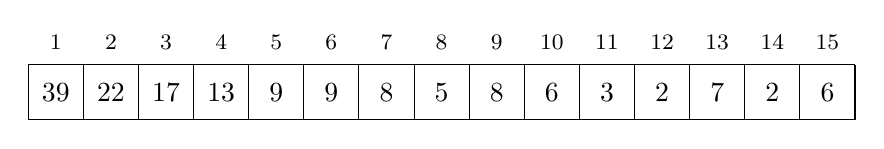
\begin{tikzpicture}[scale=0.7]
\draw (0,0) grid (15,1);

\node at (0.5,0.5) {$39$};
\node at (1.5,0.5) {$22$};
\node at (2.5,0.5) {$17$};
\node at (3.5,0.5) {$13$};
\node at (4.5,0.5) {$9$};
\node at (5.5,0.5) {$9$};
\node at (6.5,0.5) {$8$};
\node at (7.5,0.5) {$5$};
\node at (8.5,0.5) {$8$};
\node at (9.5,0.5) {$6$};
\node at (10.5,0.5) {$3$};
\node at (11.5,0.5) {$2$};
\node at (12.5,0.5) {$7$};
\node at (13.5,0.5) {$2$};
\node at (14.5,0.5) {$6$};

\footnotesize
\node at (0.5,1.4) {$1$};
\node at (1.5,1.4) {$2$};
\node at (2.5,1.4) {$3$};
\node at (3.5,1.4) {$4$};
\node at (4.5,1.4) {$5$};
\node at (5.5,1.4) {$6$};
\node at (6.5,1.4) {$7$};
\node at (7.5,1.4) {$8$};
\node at (8.5,1.4) {$9$};
\node at (9.5,1.4) {$10$};
\node at (10.5,1.4) {$11$};
\node at (11.5,1.4) {$12$};
\node at (12.5,1.4) {$13$};
\node at (13.5,1.4) {$14$};
\node at (14.5,1.4) {$15$};
\end{tikzpicture}
\end{center}
Sử dụng biểu diễn này,
cha của $\texttt{tree}[k]$
là $\texttt{tree}[\lfloor k/2 \rfloor]$,
và các con của nó là $\texttt{tree}[2k]$
và $\texttt{tree}[2k+1]$.
Lưu ý rằng điều này ngụ ý rằng vị trí của một nút
là chẵn nếu nó là con trái và lẻ nếu nó là con phải.

Hàm sau
tính giá trị của $\texttt{sum}_q(a,b)$:
\begin{lstlisting}
int sum(int a, int b) {
    a += n; b += n;
    int s = 0;
    while (a <= b) {
        if (a%2 == 1) s += tree[a++];
        if (b%2 == 0) s += tree[b--];
        a /= 2; b /= 2;
    }
    return s;
}
\end{lstlisting}
Hàm duy trì một đoạn
ban đầu là $[a+n,b+n]$.
Sau đó, ở mỗi bước, đoạn được di chuyển
lên một tầng cao hơn trong cây,
và trước đó, các giá trị của các nút không
thuộc đoạn cao hơn được cộng vào tổng.

Hàm sau tăng giá trị của mảng
tại vị trí $k$ lên $x$:
\begin{lstlisting}
void add(int k, int x) {
    k += n;
    tree[k] += x;
    for (k /= 2; k >= 1; k /= 2) {
        tree[k] = tree[2*k]+tree[2*k+1];
    }
}
\end{lstlisting}
Đầu tiên, hàm cập nhật giá trị
ở tầng dưới cùng của cây.
Sau đó, hàm cập nhật giá trị của tất cả
các nút trong cây, cho đến khi nó đến
nút gốc của cây.

Cả hai hàm trên đều hoạt động
trong thời gian $O(\log n)$, bởi vì một cây đoạn
của $n$ phần tử bao gồm $O(\log n)$ tầng,
và các hàm di chuyển lên một tầng cao hơn
trong cây ở mỗi bước.

\subsubsection{Các truy vấn khác}

Cây đoạn có thể hỗ trợ tất cả các truy vấn đoạn
mà có thể chia một đoạn thành hai phần,
tính toán câu trả lời riêng cho cả hai phần
và sau đó kết hợp hiệu quả các câu trả lời.
Ví dụ về các truy vấn như vậy là
min và max, ước chung lớn nhất,
và các phép toán bit and, or và xor.

Ví dụ, cây đoạn sau
hỗ trợ các truy vấn min:

\begin{center}
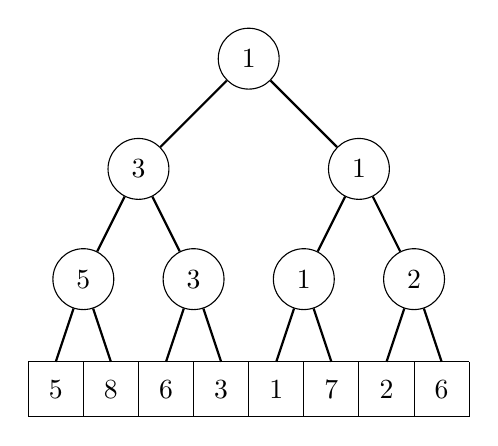
\begin{tikzpicture}[scale=0.7]
\draw (0,0) grid (8,1);

\node[anchor=center] at (0.5, 0.5) {5};
\node[anchor=center] at (1.5, 0.5) {8};
\node[anchor=center] at (2.5, 0.5) {6};
\node[anchor=center] at (3.5, 0.5) {3};
\node[anchor=center] at (4.5, 0.5) {1};
\node[anchor=center] at (5.5, 0.5) {7};
\node[anchor=center] at (6.5, 0.5) {2};
\node[anchor=center] at (7.5, 0.5) {6};

\node[draw, circle,minimum size=22pt] (a) at (1,2.5) {5};
\path[draw,thick,-] (a) -- (0.5,1);
\path[draw,thick,-] (a) -- (1.5,1);
\node[draw, circle,minimum size=22pt] (b) at (3,2.5) {3};
\path[draw,thick,-] (b) -- (2.5,1);
\path[draw,thick,-] (b) -- (3.5,1);
\node[draw, circle,minimum size=22pt] (c) at (5,2.5) {1};
\path[draw,thick,-] (c) -- (4.5,1);
\path[draw,thick,-] (c) -- (5.5,1);
\node[draw, circle,minimum size=22pt] (d) at (7,2.5) {2};
\path[draw,thick,-] (d) -- (6.5,1);
\path[draw,thick,-] (d) -- (7.5,1);

\node[draw, circle,minimum size=22pt] (i) at (2,4.5) {3};
\path[draw,thick,-] (i) -- (a);
\path[draw,thick,-] (i) -- (b);
\node[draw, circle,minimum size=22pt] (j) at (6,4.5) {1};
\path[draw,thick,-] (j) -- (c);
\path[draw,thick,-] (j) -- (d);

\node[draw, circle,minimum size=22pt] (m) at (4,6.5) {1};
\path[draw,thick,-] (m) -- (i);
\path[draw,thick,-] (m) -- (j);
\end{tikzpicture}
\end{center}

Trong trường hợp này, mỗi nút cây chứa
giá trị nhỏ nhất trong đoạn mảng
tương ứng.
Nút gốc của cây chứa giá trị nhỏ nhất
trong toàn bộ mảng.
Các thao tác có thể được cài đặt như trước đây,
nhưng thay vì tổng, giá trị nhỏ nhất được tính toán.

Cấu trúc của một cây đoạn cũng cho phép chúng ta
sử dụng tìm kiếm nhị phân để định vị các phần tử của mảng.
Ví dụ, nếu cây hỗ trợ các truy vấn min,
chúng ta có thể tìm vị trí của một phần tử
có giá trị nhỏ nhất trong thời gian $O(\log n)$.

Ví dụ, trong cây trên, một
phần tử có giá trị nhỏ nhất là 1 có thể được tìm thấy
bằng cách đi theo một đường từ nút gốc xuống dưới:

\begin{center}
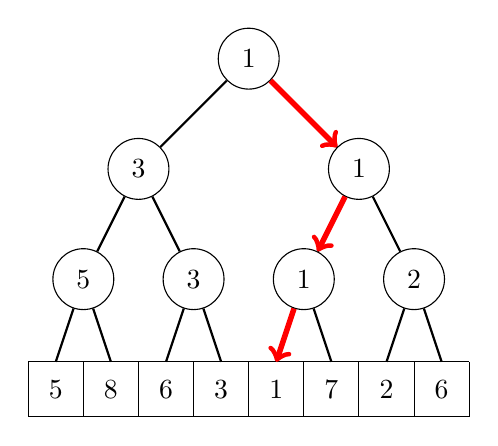
\begin{tikzpicture}[scale=0.7]
\draw (0,0) grid (8,1);

\node[anchor=center] at (0.5, 0.5) {5};
\node[anchor=center] at (1.5, 0.5) {8};
\node[anchor=center] at (2.5, 0.5) {6};
\node[anchor=center] at (3.5, 0.5) {3};
\node[anchor=center] at (4.5, 0.5) {1};
\node[anchor=center] at (5.5, 0.5) {7};
\node[anchor=center] at (6.5, 0.5) {2};
\node[anchor=center] at (7.5, 0.5) {6};

\node[draw, circle,minimum size=22pt] (a) at (1,2.5) {5};
\path[draw,thick,-] (a) -- (0.5,1);
\path[draw,thick,-] (a) -- (1.5,1);
\node[draw, circle,minimum size=22pt] (b) at (3,2.5) {3};
\path[draw,thick,-] (b) -- (2.5,1);
\path[draw,thick,-] (b) -- (3.5,1);
\node[draw, circle,minimum size=22pt] (c) at (5,2.5) {1};
\path[draw,thick,-] (c) -- (4.5,1);
\path[draw,thick,-] (c) -- (5.5,1);
\node[draw, circle,minimum size=22pt] (d) at (7,2.5) {2};
\path[draw,thick,-] (d) -- (6.5,1);
\path[draw,thick,-] (d) -- (7.5,1);

\node[draw, circle,minimum size=22pt] (i) at (2,4.5) {3};
\path[draw,thick,-] (i) -- (a);
\path[draw,thick,-] (i) -- (b);
\node[draw, circle,minimum size=22pt] (j) at (6,4.5) {1};
\path[draw,thick,-] (j) -- (c);
\path[draw,thick,-] (j) -- (d);

\node[draw, circle,minimum size=22pt] (m) at (4,6.5) {1};
\path[draw,thick,-] (m) -- (i);
\path[draw,thick,-] (m) -- (j);

\path[draw=red,thick,->,line width=2pt] (m) -- (j);
\path[draw=red,thick,->,line width=2pt] (j) -- (c);
\path[draw=red,thick,->,line width=2pt] (c) -- (4.5,1);
\end{tikzpicture}
\end{center}

\section{Các kỹ thuật bổ sung}

\subsubsection{Nén chỉ số}

Một hạn chế trong các cấu trúc dữ liệu
được xây dựng trên một mảng là
các phần tử được đánh chỉ số bằng
các số nguyên liên tiếp.
Khó khăn nảy sinh khi cần
các chỉ số lớn.
Ví dụ, nếu chúng ta muốn sử dụng chỉ số $10^9$,
mảng phải chứa $10^9$
phần tử, điều này sẽ đòi hỏi quá nhiều bộ nhớ.

\index{nén chỉ số}

Tuy nhiên, chúng ta thường có thể vượt qua hạn chế này
bằng cách sử dụng \key{nén chỉ số} (index compression),
trong đó các chỉ số ban đầu được thay thế
bằng các chỉ số $1,2,3,$ v.v.
Điều này có thể được thực hiện nếu chúng ta biết trước tất cả các chỉ số
cần thiết trong suốt thuật toán.

Ý tưởng là thay thế mỗi chỉ số ban đầu $x$
bằng $c(x)$ trong đó $c$ là một hàm
nén các chỉ số.
Chúng ta yêu cầu thứ tự của các chỉ số
không thay đổi, vì vậy nếu $a<b$, thì $c(a)<c(b)$.
Điều này cho phép chúng ta thực hiện các truy vấn một cách thuận tiện
ngay cả khi các chỉ số được nén.

Ví dụ, nếu các chỉ số ban đầu là
$555$, $10^9$ và $8$, các chỉ số mới là:

\[
\begin{array}{lcl}
c(8) & = & 1 \\
c(555) & = & 2 \\
c(10^9) & = & 3 \\
\end{array}
\]

\subsubsection{Cập nhật đoạn}

Cho đến nay, chúng ta đã cài đặt các cấu trúc dữ liệu
hỗ trợ các truy vấn đoạn và cập nhật
các giá trị đơn lẻ.
Bây giờ chúng ta hãy xem xét một tình huống ngược lại,
trong đó chúng ta nên cập nhật các đoạn và
truy xuất các giá trị đơn lẻ.
Chúng ta tập trung vào một thao tác tăng tất cả
các phần tử trong một đoạn $[a,b]$ lên $x$.

\index{mảng hiệu}

Đáng ngạc nhiên là chúng ta cũng có thể sử dụng các cấu trúc dữ liệu
được trình bày trong chương này trong tình huống này.
Để làm điều này, chúng ta xây dựng một \key{mảng hiệu} (difference array)
mà các giá trị của nó cho biết
sự khác biệt giữa các giá trị liên tiếp
trong mảng ban đầu.
Do đó, mảng ban đầu là
mảng tổng tiền tố của
mảng hiệu.
Ví dụ, hãy xem xét mảng sau:

\begin{center}
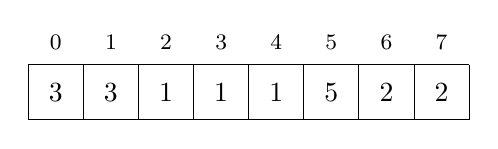
\begin{tikzpicture}[scale=0.7]
\draw (0,0) grid (8,1);

\node at (0.5,0.5) {$3$};
\node at (1.5,0.5) {$3$};
\node at (2.5,0.5) {$1$};
\node at (3.5,0.5) {$1$};
\node at (4.5,0.5) {$1$};
\node at (5.5,0.5) {$5$};
\node at (6.5,0.5) {$2$};
\node at (7.5,0.5) {$2$};


\footnotesize
\node at (0.5,1.4) {$0$};
\node at (1.5,1.4) {$1$};
\node at (2.5,1.4) {$2$};
\node at (3.5,1.4) {$3$};
\node at (4.5,1.4) {$4$};
\node at (5.5,1.4) {$5$};
\node at (6.5,1.4) {$6$};
\node at (7.5,1.4) {$7$};
\end{tikzpicture}
\end{center}

Mảng hiệu cho mảng trên như sau:
\begin{center}
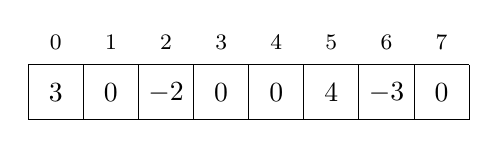
\begin{tikzpicture}[scale=0.7]
\draw (0,0) grid (8,1);

\node at (0.5,0.5) {$3$};
\node at (1.5,0.5) {$0$};
\node at (2.5,0.5) {$-2$};
\node at (3.5,0.5) {$0$};
\node at (4.5,0.5) {$0$};
\node at (5.5,0.5) {$4$};
\node at (6.5,0.5) {$-3$};
\node at (7.5,0.5) {$0$};


\footnotesize
\node at (0.5,1.4) {$0$};
\node at (1.5,1.4) {$1$};
\node at (2.5,1.4) {$2$};
\node at (3.5,1.4) {$3$};
\node at (4.5,1.4) {$4$};
\node at (5.5,1.4) {$5$};
\node at (6.5,1.4) {$6$};
\node at (7.5,1.4) {$7$};
\end{tikzpicture}
\end{center}

Ví dụ, giá trị 2 tại vị trí 6 trong mảng ban đầu
tương ứng với tổng $3-2+4-3=2$ trong mảng hiệu.

Ưu điểm của mảng hiệu là
chúng ta có thể cập nhật một đoạn
trong mảng ban đầu bằng cách chỉ thay đổi
hai phần tử trong mảng hiệu.
Ví dụ, nếu chúng ta muốn
tăng các giá trị của mảng ban đầu
giữa các vị trí 1 và 4 lên 5,
chỉ cần tăng
giá trị của mảng hiệu tại vị trí 1 lên 5
và giảm giá trị tại vị trí 5 đi 5.
Kết quả như sau:

\begin{center}
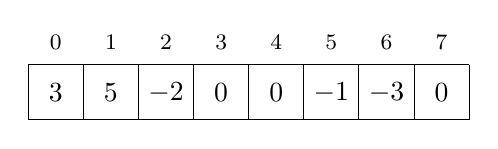
\begin{tikzpicture}[scale=0.7]
\draw (0,0) grid (8,1);

\node at (0.5,0.5) {$3$};
\node at (1.5,0.5) {$5$};
\node at (2.5,0.5) {$-2$};
\node at (3.5,0.5) {$0$};
\node at (4.5,0.5) {$0$};
\node at (5.5,0.5) {$-1$};
\node at (6.5,0.5) {$-3$};
\node at (7.5,0.5) {$0$};

\footnotesize
\node at (0.5,1.4) {$0$};
\node at (1.5,1.4) {$1$};
\node at (2.5,1.4) {$2$};
\node at (3.5,1.4) {$3$};
\node at (4.5,1.4) {$4$};
\node at (5.5,1.4) {$5$};
\node at (6.5,1.4) {$6$};
\node at (7.5,1.4) {$7$};
\end{tikzpicture}
\end{center}

Tổng quát hơn, để tăng các giá trị
trong đoạn $[a,b]$ lên $x$,
chúng ta tăng giá trị tại vị trí $a$ lên $x$
và giảm giá trị tại vị trí $b+1$ đi $x$.
Do đó, chỉ cần cập nhật các giá trị đơn lẻ
và xử lý các truy vấn tổng,
vì vậy chúng ta có thể sử dụng một cây chỉ số nhị phân hoặc một cây đoạn.

Một bài toán khó hơn là hỗ trợ cả
truy vấn đoạn và cập nhật đoạn.
Trong Chương 28, chúng ta sẽ thấy rằng ngay cả điều này cũng có thể thực hiện được.